
\subsection{Effetto del materiale sulla misura}

Abbiamo testato quanto la presenza di lastre di piombo potesse influire sulla rivelazione dei raggi cosmici. Abbiamo a disposizione il seguente materiale:
\begin{itemize}

\item 3 lastre rigide di piombo\\
spessore=\SI{4\pm1}{mm}\\
L1=\SI{39.9\pm0.1}{ cm}\\
L2=\SI{40.0\pm0.1}{cm}

\item 1 lastra di alluminio con le stesse dimensioni delle 3 precedenti

\item 10 lastre flessibili di piombo\\
spessore=\SI{2\pm1}{ mm}\\
L1=\SI{47.5\pm0.1}{ cm}\\
L2=\SI{45.0\pm0.1}{ cm}

\end{itemize}

\subsubsection{Conteggi}

Abbiamo posizionato le lastre rigide tra il PM3 ed il PM4 per vedere se esse riuscivano a fermare parte dei muoni. Per fare questa misura abbiamo confrontato le coincidenze  PM5 \& PM4 e PM5 \& PM4 \& PM3, però non possiamo confrontarle così come sono a causa dell'accettanza geometrica: anche in assenza delle lastre le coincidenze a tre sono diverse da quelle a due. Allora correggiamo le coincidenze a due con un Monte Carlo che tiene in considerazione le efficienze dei tre rivelatori. Il fattore di correzione ottenuto è il rapporto tra le accettanze delle due configurazioni  $\delta=mc(\text{PM5 \& PM4 \&PM3})/mc(\text{PM5 \& PM4})=65.71\pm0.02\%$, dove $mc$ indica il risultato del Monte Carlo per la configurazione in questione. Siano $C2$ il numero di coincidenze a due e $C3$ il numero di quelle a tre, per capire quanto sia significativo l'effetto delle lastre sulle nostre misure confrontiamo le quantità $C2'=C2 \cdot \delta$ e $C3$ in funzione del numero di lastre inserite%
\footnote{Nel grafico di \autoref{cfr} non è presente il caso di 3 lastre perché, avendone una di alluminio, abbiamo deciso di metterla insieme alla terza lastra di piombo.}. %
Dal confronto, presente in \autoref{cfr}, non si evince nessuna differenza tra i conteggi a meno di una separazione di $3\sigma$ nell'ultimo caso che, come descritto nella sezione successiva, rappresenta solo una fluttuazione.
\marginpar{scrivere il tempo di misura || $3\sigma$ l'ho detto ad occhio || giustificazione nella sezione successiva || efficienze}

\begin{figure}[h]
\centering
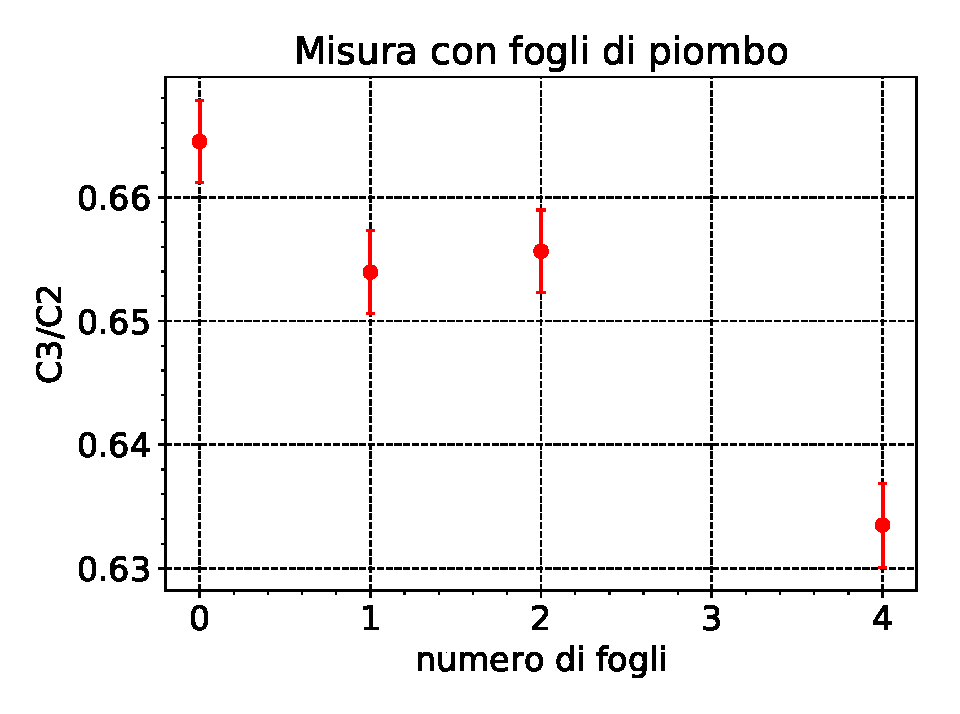
\includegraphics[width=8 cm]{confronto}
\caption{Confronto tra le coincidenze a due corrette e quelle a tre in funzione del numero di lastre inserite sul PM3.}
\label{cfr}
\end{figure}

\subsubsection{Energia}

\begin{huge}
QUI CI SAR\`A DA SCRIVERE IL VERGOGNOSO FALLIMENTO DELL'ADC
\end{huge}

Infine abbiamo eseguito due acquisizioni di lunga durata. Nella prima abbiamo messo tutte le lastre a nostra disposizione sul PM1 e abbiamo acquisito i loro rilasci di energia per tutta la notte. Il giorno seguente le abbiamo tolte ed abbiamo preso dati per \SI{4}{ore}. In entrambi i casi il trigger dell'ADC è dato dalle coincidenze PM2 \& PM1.  Abbiamo normalizzato 
\marginpar{dire che Python divide per l'area o si capisce?}
entrambi gli spettri per poterli confrontare ed evincere che non mostrano nessuna differenza, come si può vedere in \autoref{gemini}. \marginpar{non ci sono le barre d'errore sulle barre dell'istogramma}

\begin{figure}[h]
\centering
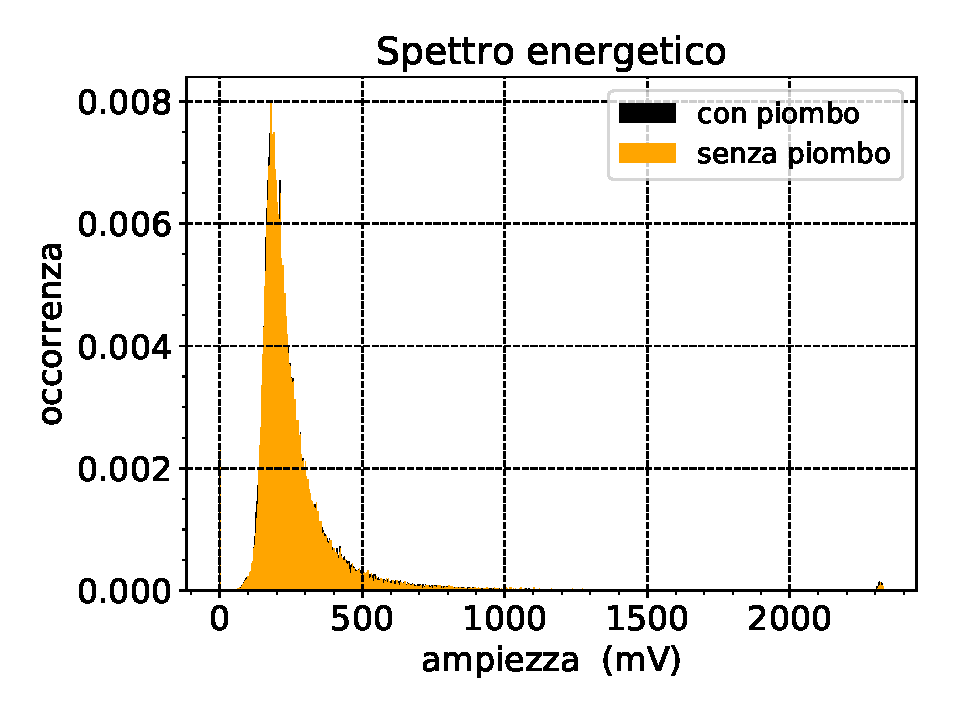
\includegraphics[width=8 cm]{gemelli}
\caption{Confronto tra gli spettri normalizzati con e senza piombo. Il picchetto a destra è dato dagli eventi talmente energetici da saturare l'uscita dell'amplificatore.}
\label{gemini}    
\end{figure}

\marginpar{solo a me la legenda fa pensare alla benzina?}
